\documentclass[12pt, a4paper, openany]{report}
\def\VersionRapport{1.0}
\usepackage[utf8]{inputenc} % un package
\usepackage[T1]{fontenc}      % un second package
\usepackage[francais]{babel}  % un troisième package
\usepackage{layout}
\usepackage[top=2.7cm, bottom=2.5cm, left=3.5cm, right=3cm]{geometry}
\usepackage{setspace}
\frenchbsetup{StandardLists=true} % à inclure si on utilise \usepackage[french]{babel}
%\usepackage{enumitem}
\usepackage[shortlabels]{enumitem}
\usepackage{amssymb}
\usepackage{color}
\usepackage{listings}
\definecolor{dkgreen}{rgb}{0,0.6,0}
\definecolor{gray}{rgb}{0.5,0.5,0.5}
\definecolor{mauve}{rgb}{0.58,0,0.82}
\definecolor{rougecerise}{rgb}{0.73,0.043,0.043}
\lstset{frame=tb,
  language=Matlab,
  aboveskip=3mm,
  belowskip=3mm,
  showstringspaces=false,
  columns=flexible,
  basicstyle={\small\ttfamily},
  keywordstyle=\color{blue},
  commentstyle=\color{dkgreen},
  stringstyle=\color{mauve},
  breaklines=true,
  breakatwhitespace=true,
  tabsize=3,
  breaklines=true,
  morekeywords={matlab2tikz},
  morekeywords=[2]{1}, 
  keywordstyle=[2]{\color{black}},
  identifierstyle=\color{black},
  numbers=left,
  numberstyle={\tiny \color{black}},
  numbersep=9pt, 
  emph=[1]{for,end,break},
  emphstyle=[1]\color{red}
}
\usepackage{multirow} % pour les tableaux
\usepackage[table]{xcolor} % pour les tableaux
\usepackage{verbatim}
%\usepackage{subcaption}
\usepackage{graphicx}
\usepackage{moreverb}
\usepackage{url}
\usepackage{pst-all}
\usepackage{eso-pic,graphicx}
\usepackage{caption} 
\usepackage[colorlinks=true,urlcolor=blue,linkcolor=red]{hyperref}
\usepackage{array}
\usepackage[toc,page]{appendix}
\usepackage[off]{auto-pst-pdf}
\usepackage{hyperref} % pour le sommaire table des matières
\AddThinSpaceBeforeFootnotes % à insérer si on utilise \usepackage[french]{babel}
\FrenchFootnotes % à insérer si on utilise \usepackage[french]{babel}
\usepackage{fancyhdr}
\pagestyle{headings}
\usepackage{pifont}  %pour les puces
\usepackage{amsmath} %pour les puces
\usepackage{subfig}
\usepackage{verbatim} % pour le code en annexe 
%%%%%%%colones 
\newcolumntype{R}[1]{>{\raggedleft\arraybackslash }b{#1}}
\newcolumntype{L}[1]{>{\raggedright\arraybackslash }b{#1}}
\newcolumntype{C}[1]{>{\centering\arraybackslash }b{#1}}
%%%%%%% 
\renewcommand{\appendixpagename}{Annexes}
\renewcommand{\appendixtocname}{Annexes}
\title{Theme: Compte Rendu Systèmes linéaires à temps discret et identification}
\author{NAIMI \bsc{Nabil} \\ KHERBICHE \bsc{Ali}}
\date{2018-2019}
%new
\newcommand{\HRule}{\rule{\linewidth}{0.5mm}}

\begin{document}

%\selectlanguage{francais}
\pagenumbering{arabic} 
\makeatletter
\begin{titlepage}
\begin{sffamily}
\begin{center}
    % Upper part of the page. The '~' is needed because \\
    % only works if a paragraph has started.
    
\includegraphics[scale=0.5]{Logo_UT3.jpg}~\\[1cm]
    \textsc{\LARGE M1 ISTR-RODECO  }\\[1cm]
    \textsc{\Large Compte Rendu Systèmes Linéaires à Temps Discret et Identification}\\[1cm]
    % Title
    \HRule \\[0.4cm] % saut de ligne
    { \huge  \textsc {Reconstruction de l'environnement d'un robot mobile à l'aide de la méthode des moindres carrés \\[0.4cm] }}

    \HRule \\[1cm]   % sous de ligne 
    
\includegraphics[scale=0.1]{logomaster.jpg}
    \\[1cm]
    % Author and supervisor
    \begin{minipage}{0.4\textwidth}
      \begin{flushleft} \large
         \textsc{\emph {Fait par:} \\KHERBICHE Ali\\ NAIMI Nabil}  
          \newline
          Promotion 2018-2019 \\
      \end{flushleft}
    \end{minipage}
    \begin{minipage}{0.4\textwidth}
      \begin{flushright} \large
        %%\emph{Tuteur et}
        \emph{Tuteurs:} \textsc{Mme.Carine JAUBERTHIE\\Mme.Viviane CADENAT}
      \end{flushright}
    \end{minipage}
    \vfill
    % Bottom of the page
    {\large Mars 2018}
  \end{center}
  \end{sffamily}                
  \end{titlepage}  
\makeatother
   
%*********************** somaire **************
\renewcommand{\contentsname}{Sommaire}
\tableofcontents
%*********************** listes des figures **************
\listoffigures
%*********************** listes des tableaux **************
%\listoftables

\chapter*{\textsc{Introduction}}
\addcontentsline{toc}{chapter}{\textsc{Introduction}}

	\paragraph{}
	L'objectif de cette séance est d'étudier le problème de la localisation d'un robot mobile (Pekee II). Nous traiterons ce problème par la méthode des moindres carrés récursifs.
	
	\begin{center}
	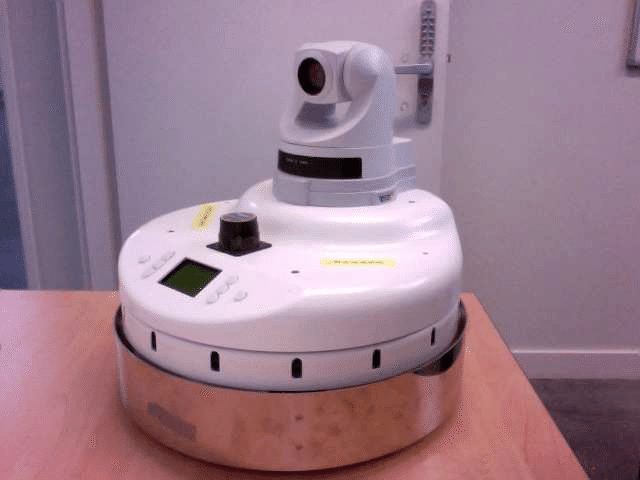
\includegraphics[scale=0.5]{pekee.png}
	\captionof{figure}{\textit{Robot pekee II\\}}
	\label{fig1} 
	\end{center}   
	
\chapter{\textsc{Reconstruction de l'environnement}}
%\addcontentsline{toc}{chapter}{\textsc{Reconstruction de l'environnement}}

\section{\textsc{Tracé des données}}

	\paragraph{}
	D'après le graphe ci-dessous qui provient du fichier ZT, l'axe des ordonnées correspond à la première colonne 			qui est en fonction de la deuxième celle ci correspond aux abscisses. On constate que le laser fournit un 				ensemble de points sous forme de deux pseudo-droites qu'on pourra modéliser en droites par la méthode des 				moindres carrés.\\  
	
	\begin{center}
	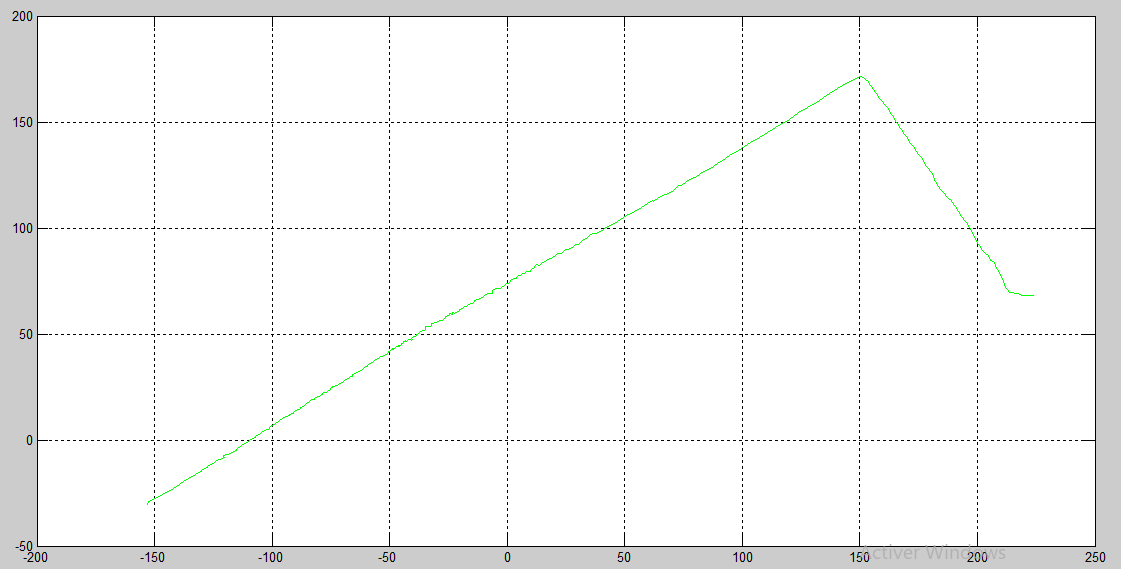
\includegraphics[scale=0.5]{graphedonnees.png}
	\captionof{figure}{\textit{Tracé des données du robot\\}}
	\label{fig2} 
	\end{center} 

\pagebreak
\section{\textsc{Identification par les moindres carrés basiques}}	

	\paragraph{}
	On sait que l'équation d'une droite est de la forme $ y=ax+b $ qu'on pourra illustrer aussi de cette manière :\\
	\begin{center}
		$ y = \begin{bmatrix} x&1 \end{bmatrix} \begin{bmatrix} a\\b \end{bmatrix} $ 
	\end{center}
	
	Arrivés là une identification avec la forme $ y = \varphi^{T}P $ est possible avec :
	  
	\begin{center}
		$ \varphi^{T} = \begin{bmatrix} x&1 \end{bmatrix} $ et $ P = \begin{bmatrix} a\\b \end{bmatrix}$
	\end{center}
	Ou $P$ correspond aux paramètres et $\varphi^{T}$ correspond au vecteur de régression. Le fichier ZT contient 			deux colonnes: colonne 1 pour les Y et colonne 2 	pour les X, donc on aura exactement N=507 mesures alors on 			parle de matrice de régression $\phi$ et pas que de vecteur de régression $\varphi$, avec $ \phi = 					\begin{bmatrix} \varphi^{T}_{1}\\.\\ \varphi^{T}_{i} \\.\\ \varphi^{T}_{N} \end{bmatrix} $ et $ Y = 					\begin{bmatrix} y_{1}\\.\\ y_{i} \\.\\ y_{N} \end{bmatrix} $ ,\label{section 1.2} \hyperref[Annexe A] {voir code 	Matlab en annexe}.
	
	\begin{center}
	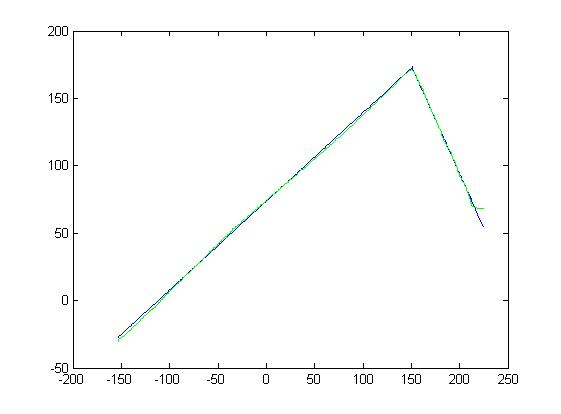
\includegraphics[scale=0.7]{2.jpg}
	\captionof{figure}{\textit{Tracé des droites modélisées par les MC basiques superposé avec celui des données\\}}
	\label{fig3} 
	\end{center}

	\textbf{Nota:} La détection de l'instant de commutation à i=417 nous a permis de tracer les deux modéles. \\[1cm] 
	
	\par Cette approche est limitée car elle traite un mur à la fois, autrement dit un modèle par mur. Mais comme la problématique abordée comporte plus d'un mur l'algorithme de cette approche risque d'être très long et quasiment impossible à coder pour une situation réelle ou on affronte une multitude d'obstacles (murs...etc). 
	

\section{\textsc{Identification par les moindres carrés récursifs}}
\subsection{\textsc{ Principe et ... }}

	\paragraph{} L'algorithme des moindres carrés récursifs se compose de deux parties, partie initialisation et partie calcul itératif des parmaètres. Il existe deux solutions pour initialiser cet algorithme, soit avec un choix arbitraire des paramètres ou bien de faire un petit prélévement des mesures donc celles du fichier ZT. Dans notre cas on se penchera plus tôt sur la deuxième option c'est à dire on prélève un nombre de mesures $N_0$ qui est égale dans notre cas à $3$ puis en utilisant les moindres carrés basiques on poura facilement trouver la matrice de régression $\phi_0$ ainsi que les paramètres $P_0$ et la matrice $A_0$ qui est égale à $\phi^{T}_{0} \phi_0$.\\
Le calcul itératif des paramètres consiste à acquérir à chaque itération une nouvelle mesure $y_{N+1}$, de calculer son $y_{MOD_{N+1}} = \varphi^{T}_{N+1} \hat{P}_N$
, \label{section 1.3.1} \hyperref[Annexe B] {voir code Matlab en annexe}. 
%\input{chap2.tex}
%\input{chap4&5.tex}
%\input{conclusion.tex}
\begin{appendices}
\chapter*{\textsc{Annexe A}}
	\addcontentsline{toc}{chapter}{\textsc{Annexe A}}		
	
	Code MATLAB pour les moindres carrés basiques ,\label{Annexe A} \hyperref[section 1.2]{cliquer pour retourner vers section 1.2}.

	\begin{lstlisting}	
	 
clc
clear all
close all

load donnees.mat

M=417; % instant de commutation
k=1;
u=1;
o=1;
ov=1;
e=1;
p=1;
f=1;
d=1;
oo=1;
dd=1;
ii=1;
ddd=1;
ooo=1;
iii=1;
H=507;

% MC basiques de la droite 1 
for i=1:M+1
A1(o,:)= [ZT(i,2) 1]; % phi = A
y1(i)=ZT(i,1);
o= o+1;
end

% MC basiques pour la droite 2
for j=M+1:H
A2(e,:)= [ZT(j,2) 1];
y2(f)=ZT(j,1);
e= e+1;
f=f+1;
end

C1=inv(A1'*A1)*A1'*y'; % P1 chapeau
C2=inv(A2'*A2)*A2'*y'; % P2 chapeau

for i=1:M+1
ZT1(i)= C1(1)*ZT(i,2)+C1(2);
end

for i=M+1:H
ZT2(d)= C2(1)*ZT(i,2)+C2(2);
d=d+1;
end

plot(ZT(1:M+1,2),ZT1') % plot de la 1ere droite
hold on
plot(ZT(M+1:H,2),ZT2') % plot de la 2eme droite
hold on
plot (ZT(:,2),ZT(:,1),'g') % plot des donnees
hold on

	\end{lstlisting}
	
	\chapter*{\textsc{Annexe B}}
	\addcontentsline{toc}{chapter}{\textsc{Annexe B}}		
	
	\label{Annexe B} \hyperref[section 1.3.1]{ Cliquer pour retourner vers section 1.3.1}.

	\begin{lstlisting}	
	 
for i=1:3 %%  Prise des trois premieres mesures pour la 1ere courbe 
phiz(oo,:)= [ZT(i,2) 1]; % calcul de phi_zero de la droite 1
yr1(oo)=ZT(i,1);
oo= oo+1;
end

Az1= phiz'*phiz; % A_zero de la droite 1
az1=Az1; % pour la question 3.c

 % Calcul du P01 chapeau initial a laide des MC basiques
 Cr1=inv(phiz'*phiz)*phiz'*yr1';
cr1=Cr1; % pour la question 3.c
invAz1 = inv (Az1);
invaz1=invAz1; % pour la question 3.c

 %Prise des trois premieres mesures apres l'instant de commutation pour la 2eme courbe 
for i=M:M+2
phiz2(ooo,:)= [ZT(i,2) 1]; % calcul de phi_zero de la droite 2
yr2(ooo)=ZT(i,1);
ooo= ooo+1;
end

Az2= phiz'*phiz2; % A_zero de la droite 2
Cr2=inv(phiz2'*phiz2)*phiz2'*yr2';% P02 chapeau
invAz2 = inv (Az2);

for i=1:M+1 % application de MC recursifs pour la 1ere droite
yr1mod=[ZT(i,2) 1]*Cr1;
Kn1plus = (invAz1*[ZT(i,2) 1]')/(1+[ZT(i,2) 1]*(invAz1*[ZT(i,2) 1]')); %KN+1
invAz1 = invAz1 - Kn1plus*[ZT(i,2) 1]*invAz1; % l'inverse de AN+1
Cr1= Cr1 + Kn1plus*(ZT(i,1) - yr1mod); %PN+1 chapeau 
end

for i=M+1:H % application de MC recursifs pour la 2eme droite
yr2mod=[ZT(i,2) 1]*Cr2;
YR2MOD(iii)=yr2mod;
Kn2plus = (invAz2*[ZT(i,2) 1]')/(1+[ZT(i,2) 1]*(invAz2*[ZT(i,2) 1]'));
invAz2 = invAz2 - Kn2plus*[ZT(i,2) 1]*invAz2;
Cr2= Cr2 + Kn2plus*(ZT(i,1) - yr2mod);
end

for i=1:M+1
ZTr1(dd)= Cr1(1)*ZT(i,2)+Cr1(2);
dd=dd+1;
end

for i=M+1:H
ZTr2(ddd)= Cr2(1)*ZT(i,2)+Cr2(2);
ddd=ddd+1;
end

plot(ZT(1:M+1,2),ZTr1,'r')
hold on
plot(ZT(M+1:H,2),ZTr2,'r')
grid on
	 
	\end{lstlisting}

\chapter*{\textsc{Annexe C}}
	\addcontentsline{toc}{chapter}{\textsc{Annexe C}}
	
	\label{Annexe C} \hyperref[section 1.3.2] {Cliquer pour retourner vers section 1.3.2 }.
	
	\begin{lstlisting}	
clc
clear all
close all
load donnees.mat
% Question 2
M=417;
k=1;
u=1;
o=1;
ov=1;
e=1;
p=1;
f=1;
d=1;
oo=1;
dd=1;
ii=1;
ddd=1;
ooo=1;
iii=1;
H=507;	

for i=1:3 %% 1ere courbe
phiz(oo,:)= [ZT(i,2) 1];
yr1(oo)=ZT(i,1);
oo= oo+1;
end
Az1= phiz'*phiz;
az1=Az1; % pour la question 3.c
Cr1=inv(phiz'*phiz)*phiz'*yr1';%% P01 chapeau
cr1=Cr1; % pour la question 3.c
invAz1 = inv (Az1);
invaz1=invAz1; % pour la question 3.c
 
for i=1:H
Y1=[ZT(i,1)];
Y1mod=[ZT(i,2) 1]*cr1;
Kn1p = (invaz1*[ZT(i,2) 1]')/(1+[ZT(i,2) 1]*(invaz1*[ZT(i,2) 1]'));
invaz1 = invaz1 - Kn1p*[ZT(i,2) 1]*invaz1;
cr1= cr1 + Kn1p*(ZT(i,1) - Y1mod);
err(i) = abs(Y1-Y1mod); % calcul de l'erreur de prediction pour chaque iteration
if(err(i)>4) 	
 	v=i;
 	break;
end
end
		
for i=1:v-2
zt1(i)= cr1(1)*ZT(i,2)+cr1(2);
end	

plot(ZT(1:v-2,2),zt1,'m')
hold on
plot (ZT(:,2),ZT(:,1),'g')
grid on		
	\end{lstlisting}
	
	\chapter*{\textsc{Annexe D}}
	\addcontentsline{toc}{chapter}{\textsc{Annexe D}}
	
	\label{Annexe D} \hyperref[section 1.3.3] {Cliquer pour retourner vers section 1.3.3 }.
	
	\begin{lstlisting}
clc
clear all
close all
load donnees.mat

M=417;
k=1;
u=1;
o=1;
ov=1;
e=1;
p=1;
f=1;
d=1;
oo=1;
dd=1;
ii=1;
ddd=1;
ooo=1;
iii=1;
H=507;

for i=1:3 %% 1ere courbe
phiz(oo,:)= [ZT(i,2) 1];
yr1(oo)=ZT(i,1);
oo= oo+1;
end
Az1= phiz'*phiz;
az1=Az1; % pour la question 3.c
Cr1=inv(phiz'*phiz)*phiz'*yr1';%% P01 chapeau
cr1=Cr1; % pour la question 3.c
invAz1 = inv (Az1);
invaz1=invAz1; % pour la question 3.c
	
i = 0;
j=1;
Niter=88;
result=0;
error=0;
for i=1:507
Y1=[ZT(i,1)];
Y1mod=[ZT(i,2) 1]*cr1;
Kn1p = (invaz1*[ZT(i,2) 1]'/(1+[ZT(i,2) 1]*(invaz1*[ZT(i,2) 1]'));
invaz1 = invaz1 - Kn1p*[ZT(i,2) 1]*invaz1;
cr1= cr1 + Kn1p*(ZT(i,1) - Y1mod);
err= abs(Y1-Y1mod);

if (err>4)
v=i;

for(j=v:H-Niter)
for (k=v:v+Niter-1)

error=err;
if(error>4)
result=result+1;
end
if (result==Niter)
for s=1:3
fiz(ov,:)= [ZT(s+i,2) 1];
Yr2(ov)=ZT(s+i,1);
ov= ov+1;
end
az2= fiz'*fiz;
cr2=inv(fiz'*fiz)*fiz'*Yr2';
invaz2 = inv (az2);
for u=1:507-i
Y2mod=[ZT(u+i,2) 1]*cr2;
Kn2p = (invaz2*[ZT(i+u,2) 1]')/(1+[ZT(i+u,2)
1]*(invaz2*[ZT(i+u,2) 1]'));
invaz2 = invaz2 - Kn2p*[ZT(i+u,2) 1]*invaz2;
cr2= cr2 + Kn2p*(ZT(i+u,1) - Y2mod);
end
end
end
v=v+1;
end
break
end
end

for i=1:v-2
zt1(i)= cr1(1)*ZT(i,2)+cr1(2);
end
sd=1;
for i=v-2:H
zt2(sd)= cr2(1)*ZT(i,2)+cr2(2);
sd=sd+1;
end

plot(ZT(1:v-2,2),zt1,'m')
hold on
plot(ZT(v-2:H,2),zt2,'m')
hold on
plot (ZT(:,2),ZT(:,1),'g')
grid on						
	\end{lstlisting}
		
	\chapter*{\textsc{Annexe E}}
	\addcontentsline{toc}{chapter}{\textsc{Annexe E}}
	
	\label{Annexe E} \hyperref[section 1.3.4] {Cliquer pour retourner vers section 1.3.4 }.
	
	\begin{lstlisting}	
clc
clear all
close all
load donnees.mat

M=417;
k=1;
u=1;
o=1;
ov=1;
e=1;
p=1;
f=1;
d=1;
oo=1;
dd=1;
ii=1;
ddd=1;
ooo=1;
iii=1;
H=507;

A0=15000*eye(2); % choix arbitraire de la matrice A0
a0=A0;
P0= [12;5];% choix arbitraire des parametres
p0=[150;200]; 
i = 0;
j=1;
Niter=88;
result=0;
error=0;

for i=1:507
Y1=[ZT(i,1)];
Y1mod=[ZT(i,2) 1]*P0;
Kn1p = (A0*[ZT(i,2) 1]')/(1+[ZT(i,2) 1]*(A0*[ZT(i,2) 1]'));
A0 =A0 - Kn1p*[ZT(i,2) 1]*A0;
P0= P0 + Kn1p*(ZT(i,1) - Y1mod);
err= abs(Y1-Y1mod);


if (err>4)
v=i;

for(j=v:H-Niter)
for (k=v:v+Niter-1)
error=err;
if(error>4)
result=result+1;
end
if (result==Niter)

A01=10000*eye(2);
P01= [5;18];
for u=1:507-i
Y2mod=[ZT(u+i,2) 1]*P01;
Kn2p = (A01*[ZT(i+u,2) 1]')/(1+[ZT(i+u,2)
1]*(A01*[ZT(i+u,2) 1]'));
A01 = A01 - Kn2p*[ZT(i+u,2) 1]*A01;
P01= P01 + Kn2p*(ZT(i+u,1) - Y2mod);
end
end
end
v=v+1;
end
break
end
end

for i=1:v-2
zt1(i)= A0(1)*ZT(i,2)+A0(2);
end

for i=v:507
Y1=[ZT(i,1)];
Y1mod=[ZT(i,2) 1]*p0;
Kn1p = (a0*[ZT(i,2) 1]')/(1+[ZT(i,2) 1]*(a0*[ZT(i,2) 1]'));
a0 =a0 - Kn1p*[ZT(i,2) 1]*a0;
p0= p0 + Kn1p*(ZT(i,1) - Y1mod);
end
sd=1;
for i=v+2:H
zt2(sd)= a0(1)*ZT(i,2)+a0(2);
sd=sd+1;
end
plot(ZT(1:v-2,2),zt1,'m')

hold on
plot(ZT(v+2:H,2),zt2,'m')
hold on
plot (ZT(:,2),ZT(:,1),'g')
grid on				
	\end{lstlisting}
	
\end{appendices}

%*********************** Bibliographie ************ 
\bibliographystyle{alpha}
\bibliography{biblio}  



\end{document}
